 \thispagestyle{gocconone}
\pagestyle{gocco}
\everymath{\color{gocco}}
\graphicspath{{../gocco/pic/}}
\blfootnote{$^1$\color{gocco}Hà Nội.}
\blfootnote{\color{gocco}$^2$Một kiểu lãnh chúa Ấn Độ.}
\blfootnote{\color{gocco}$^3$Phiên bản Ấn Độ của cờ vua có luật chơi hơi khác so với cờ vua phương Tây.}
\begingroup
\AddToShipoutPicture*{\put(0,616){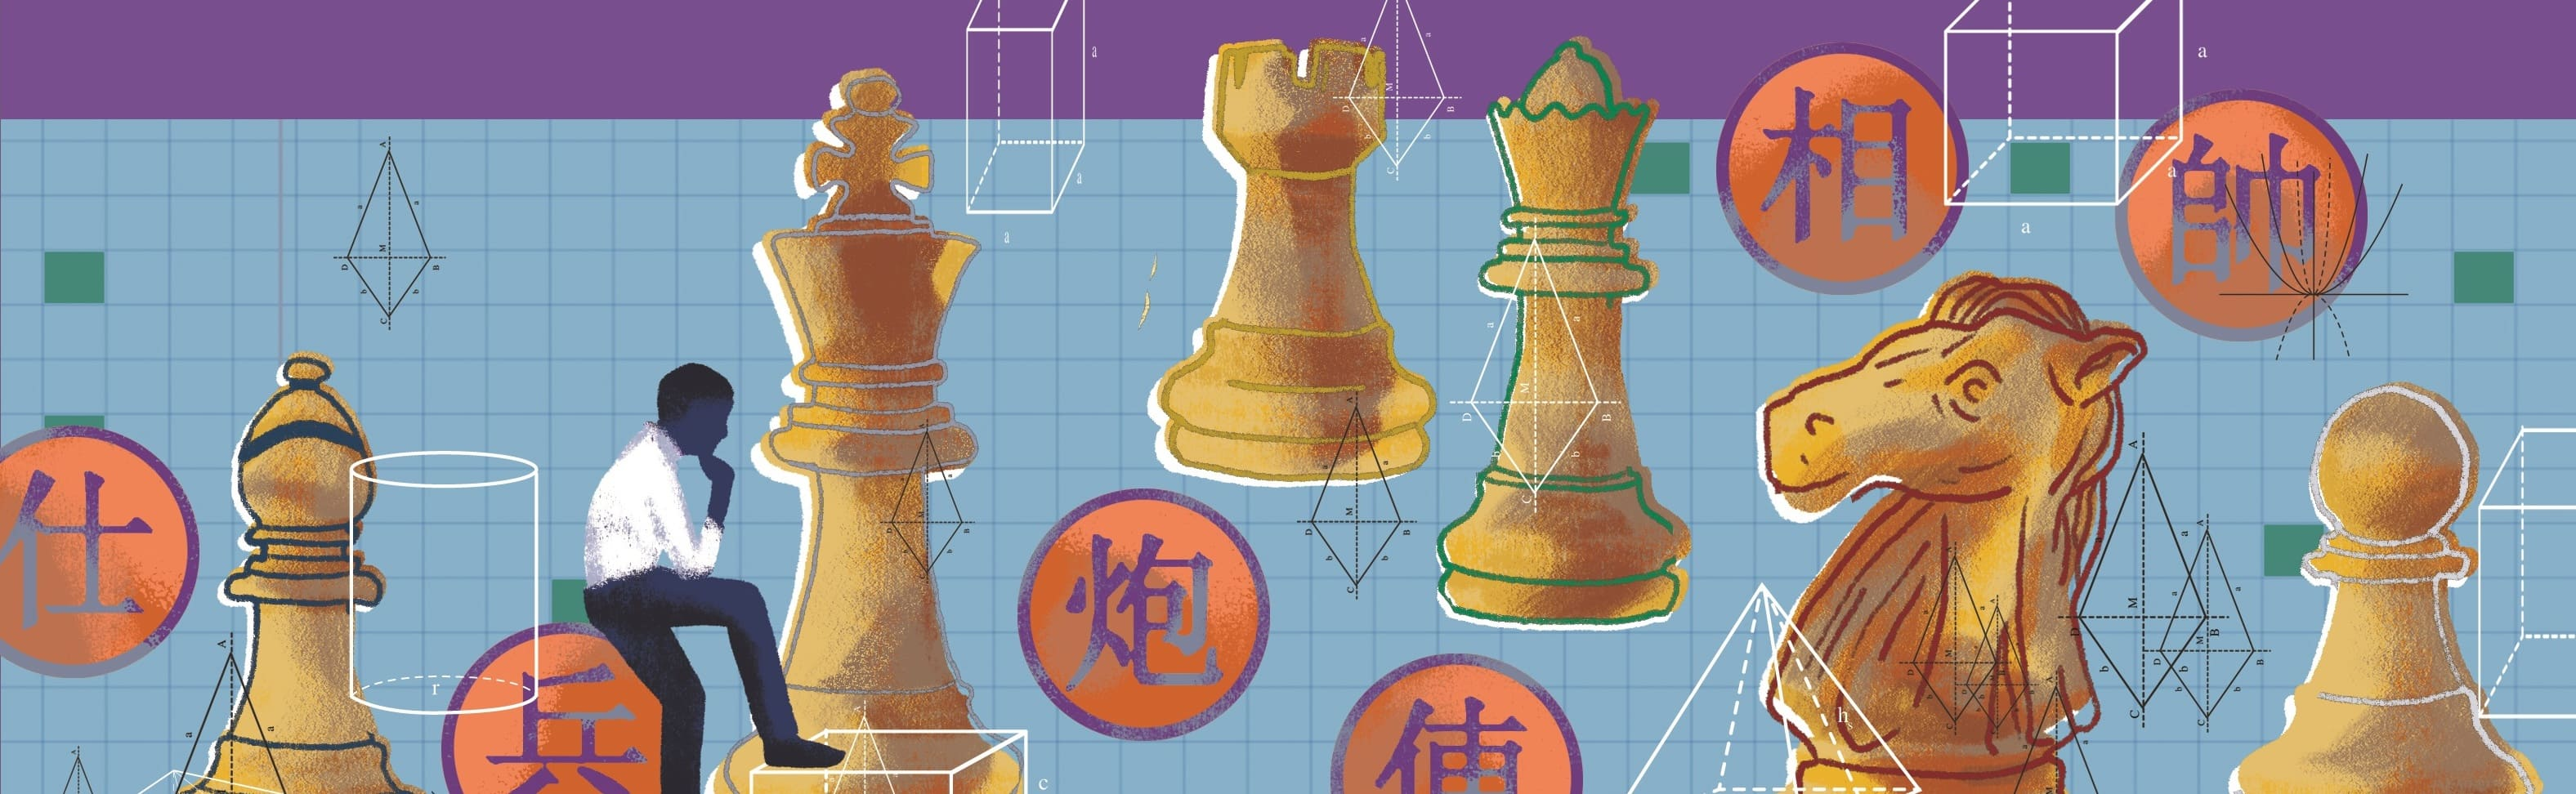
\includegraphics[width=19.3cm]{../bannergocco}}}
\AddToShipoutPicture*{\put(56,536){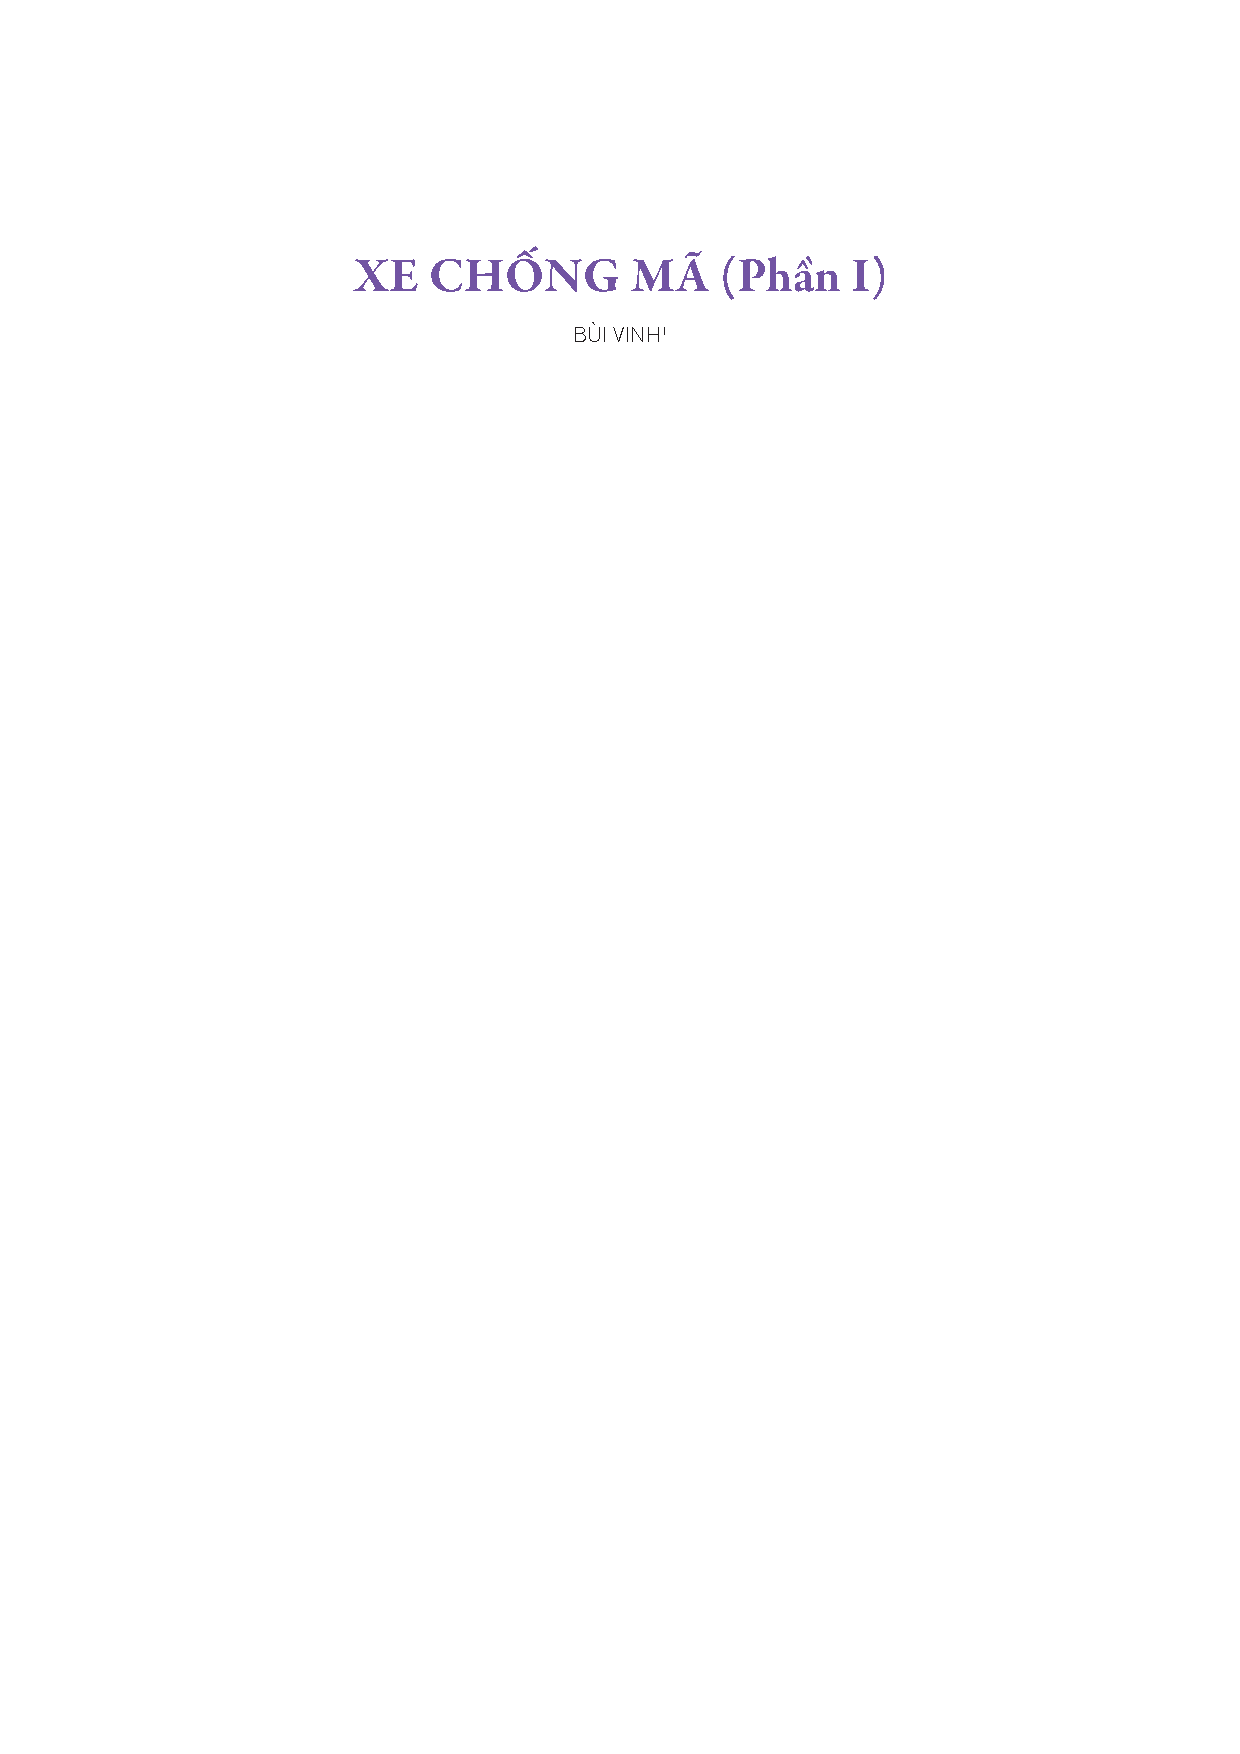
\includegraphics[scale=0.9]{../tieude2.pdf}}} 
\centering
\endgroup

\vspace*{170pt}
\begin{multicols}{2}
	Trong bất kỳ môn thể thao nào, khán giả cũng thích chứng kiến một vận động viên vô danh đột ngột xuất hiện và lật đổ các nhà vô địch. Nhưng ngày nay, với sự chuyên nghiệp hóa trong hầu hết các khía cạnh, điều đó có lẽ chỉ xảy ra trong các bộ phim hay các cuốn tiểu thuyết. Đặc biệt, nó gần như không thể xảy ra trong cờ vua, nơi bạn cần phải trải qua rất nhiều khổ luyện trước khi có đủ năng lực để thi đấu ngang bằng với các đại kiện tướng. Và không phi thường sao nếu như một người chưa bao giờ học chơi cờ vua một cách bài bản, chỉ dựa vào duy nhất tài năng của mình, mà trở thành nhà vô địch thế giới, như trong \textit{Thiên truyện cờ vua} của Stefan Zweig?
	\vskip 0.05cm
	Đó chính là điều mà một người đã làm được vào những năm $1930$: ông đã đánh bại Capablanca (người khi đó tuy không còn giữ chức vô địch thế giới, nhưng vẫn còn đang trong thời kỳ đỉnh cao của sự nghiệp), cũng như cả các kỳ thủ Frank Marshall và Tartakover. Ngoài ra, ông cũng cầm hòa Alekhine, nhà đương kim vô địch thế giới, và với Max Euwe, nhà vô địch thế giới tiếp theo, mà không hề học một chút gì về khai cuộc, không biết gì về lịch sử cờ vua hay lối chơi của các đối thủ và thậm chí, trong đa số các ván đấu của mình không hề ... nhập thành!
	\vskip 0.1cm
	Sẽ chẳng ai tin một câu chuyện như vậy nếu xem nó trong rạp chiếu phim nhưng Sultan Khan đã làm được tất cả những điều đó! Đặc biệt hơn nữa, ông là một người hầu của Ngài Umar, một maharaja$^2$ của vùng Punjab, Ấn Độ (ngày nay thuộc về Pakistan). Khi theo hầu Ngài Umar đến Anh vào năm $1929$, ông $24$ tuổi và là kỳ thủ mạnh nhất trong cờ vua Ấn Độ$^3$ ở vùng Punjab. Theo yêu cầu của người chủ, ông học luật chơi của của cờ vua phương Tây.
	\begin{figure}[H]
		\vspace*{-5pt}
		\centering
		\captionsetup{labelformat= empty, justification=centering}
		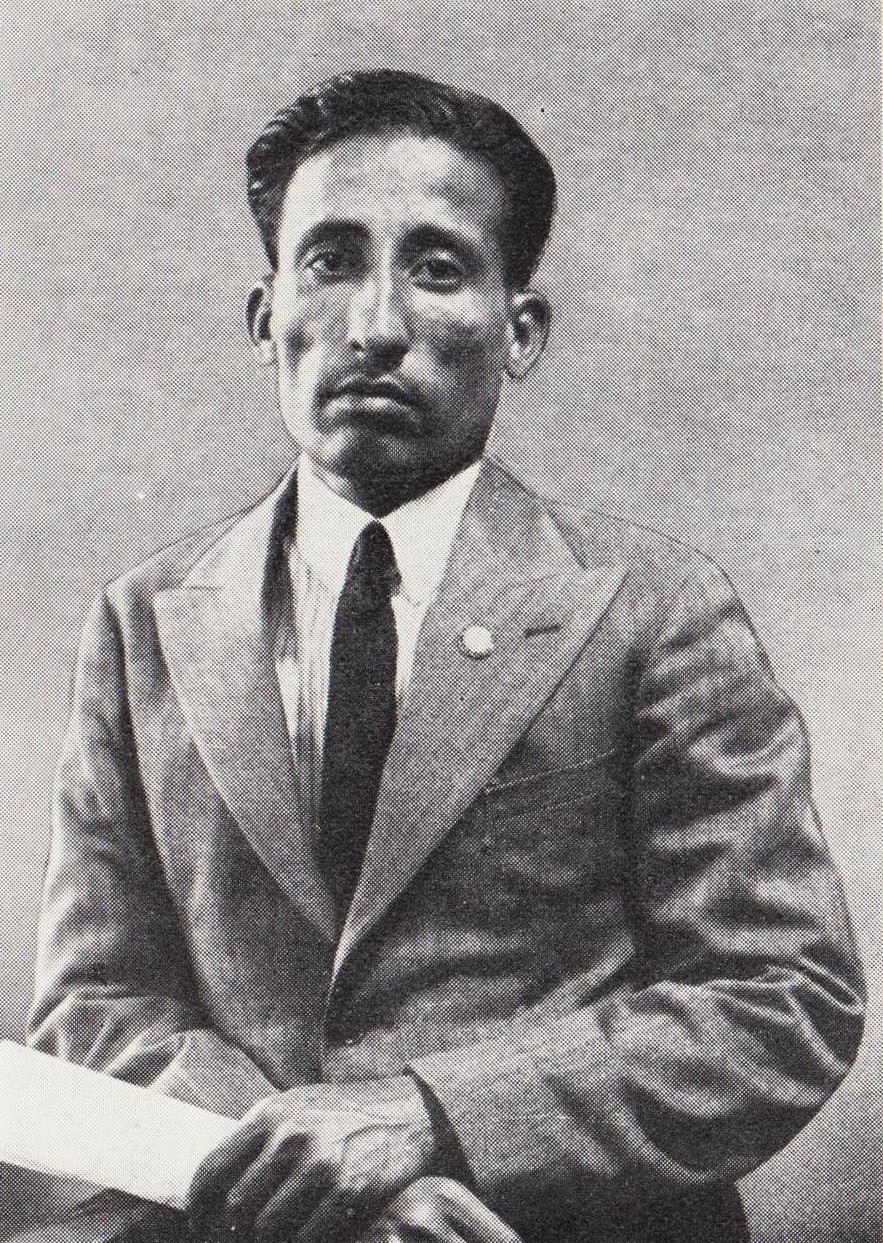
\includegraphics[width= 0.58\linewidth]{1}
		\caption{\small\textit{\color{gocco}Sultan Khan ($1903-1966$) kỳ thủ cờ vua người Ấn Độ (về sau thuộc về Pakistan).}}
		\vspace*{-10pt}
	\end{figure}
	Khi đến Anh, ông đã giành được chức vô địch Đế chế Anh năm $1929$ ngay từ lần đầu tiên tham gia, trước sự sửng sốt của mọi người (về sau, ông còn tiếp tục giành chức vô địch vào các năm $1932$ và $1933$). Vì không có luật nhập thành trong cờ vua Ấn Độ, ông đã chơi nhiều ván mà không nhập thành, trong đó có cả ván cờ thắng Capablanca hoặc trong ván cờ hòa với Alekhine. Ngay cả những năm $1930$, nếu không thuộc các thế khai cuộc trong cờ vua thì gần như không thể chơi ở các giải đấu đỉnh cao. Nhưng Sultan Khan chưa từng học lý thuyết về cờ, cũng như không đọc bất kỳ cuốn sách nào, do mù chữ. Mặc dầu vậy, tài năng thiên phú của ông đã bù đắp cho những sự thiếu hiểu biết này về khai cuộc khi các ván cờ đi tới trung cuộc. Ông cũng có một trực giác rất nhạy bén về tàn cuộc mặc dù cũng không biết gì về lý thuyết tàn cuộc. Một điều thú vị nữa là ông cũng không có ý thức gì về việc tính toán lợi ích vật chất và vinh quang: tại giải Hastings năm $1931$, sau ván thắng huyền thoại trước Capablanca, ông có cơ hội giành chiến thắng chung cuộc giải này bằng cách hòa trong ván đấu với Max Euwe, nhưng ông từ chối đề nghị hòa của Euwe và sau đó để thua! Có lẽ là vì đề nghị hòa không có trong thế giới của ông. Kiểu như: ``Ván cờ đang thú vị, tại sao lại dừng lại?"
	\vskip 0.1cm
	Năm $1933$, ông theo người chủ trở lại Ấn Độ và không còn cơ hội để chơi cờ vua nữa và nhanh chóng bị rơi vào quên lãng. Chỉ nhiều năm sau khi qua đời (vào năm $1966$), ông mới được giới cờ vua biết đến. Ngài Umar đã chấm dứt sự nghiệp của người mà, có lẽ, nếu được đào tạo chuyên nghiệp có thể đã trở thành một trong những kỳ thủ cờ vua vĩ đại nhất mọi thời đại. Tất nhiên, không ai chắc được rằng liệu ông có thể giành chức vô địch thế giới hay không, nhưng với những gì ông đã đạt được chỉ sau $4$ năm ở Anh, điều đó không phải là không thể. 
	\vskip 0.1cm
	Một số thành tích nổi bật của Sultan Khan:  
	\vskip 0.1cm
	$\bullet$	Vô địch Đế chế Anh các năm $1929$, $1932$ và $1933$;
	\vskip 0.1cm 
	$\bullet$	Đứng thứ hai (sau Tarktakower) tại giải Liege năm $1930$;
	\vskip 0.1cm 
	$\bullet$	Đứng thứ ba tại giải Hastings năm $1930-1931$ (sau nhà vô địch thế giới tương lai Max Euwe và cựu vô địch thế giới Capablanca);
	\vskip 0.1cm
	$\bullet$	Hạ Savielly Tartakower $6{.}5-5{.}5$ trong một trận đấu vào tháng $1$ năm $1931$;
	\vskip 0.1cm
	Sau đây là diễn biến ván đấu nổi tiếng Khan--Capablanca tại giải Hastings $1930-1931$.
	\vskip 0.1cm
	\textbf{\color{gocco}Sultan Khan -- Capablanca}
	\vskip 0.1cm
	\textbf{\color{gocco}$1.$ Mf$3$ Mf$6$ $2.$ d$4$ b$6$ $3.$ c$4$ Tb$7$ $4.$ Mc$3$ e$6$ $5.$ a$3$}. Một nước đi tiên phong. Nhiều thập kỷ sau, nó được gọi là biến thể Petrosian, một khai cuộc ưa thích của Garry Kasparov. Cho dù một vài kỳ thủ đã thử khai cuộc  này vào những năm $1920$ nhưng gần như chắc chắn là Sultan Khan không biết khai cuộc này. Sự thiếu hiểu biết này của Khan đã tạo cơ hội cho sự sáng tạo của ông. Ông đã thử nghiệm những nước đi ngắn cho Tốt như vậy ở cả hai cánh (a$3$ và h$3$) trong một số ván khác, nhưng ở ván này là hiệu quả nhất. Đen bị ngăn không cho Tượng di chuyển đến b$4$, và do đó Trắng giành được nhiều quyền kiểm soát hơn đối với e$4$. $5$... d$5$ $6.$ cxd$5$ exd$5$. Như người ta chờ đợi từ Capablanca, một nước đi cổ điển, duy trì một Tốt ở trung tâm. Nước này hoàn toàn có thể chơi được, nhưng biến thể chính hiện đại là $6$...Mxd$5$. \textbf{\color{gocco}$7.$ Tg$5$ Te$7$ $8.$ e$3$ $0-0$ $9.$ Td$3$ Me$4$}. Capablanca cho thấy ý định đổi quân nhanh chóng. $9$...Mbd$7$, để hoàn thiện phát triến là nước đi tốt hơn. $10.$ Tf$4$! Mặc dù thiếu kinh nghiệm trong khai cuộc, Khan cho thấy sự thấu hiểu thế trận. Thay vì \textbf{\color{gocco}$10$ Txe$7$ Hxe$7$}, điều này sẽ giải phóng thế trận của Đen do khi đó Hậu thoát khỏi hàng sau và các Xe sẵn sàng tiến vào giữa bàn cờ. $10$... Md$7$ $11.$ Hc$2$. Một nước đi tuyệt vời, nhằm vào hai ô nhạy cảm của Đen, h$7$ và c$7$. Trong trường hợp này, thói quen trì hoãn nhập thành của Khan được đền đáp. $11$... f$5$.
	\vskip 0.1cm
	[$11$... Mxc$3$? $12.$ Txh$7+$ Vh$8$ $13.$ bxc$3$ g$6$ $14.$ Txg$6$ fxg6 $15.$ Hxg$6$ Tf$6$ $16.$ h$4$ với thế chủ động.]
	\vskip 0.1cm
	[Về sau, Capablanca nói rằng ở đây cần phải đi nước quen thuộc $11$... Mdf$6$, tuy nhiên ông (và nhiều người khác) đã bỏ sót một chiến thuật đơn giản: \textbf{\color{gocco}$12.$ Txc$7$ Hxc$7$ $13.$ Mxe$4$ Hxc$2$ $14.$ Mxf$6+$ Txf$6$ $15.$ Txc$2$}.]
	\vskip 0.1cm
	\textbf{\color{gocco}$12.$ Mb$5$} Đen gặp khó trong việc bảo vệ Tốt c$7$. Nếu $12$... c$5$ $13$ Mc$7$ đe dọa Xe và ghim với e$6$. $12$... Td$6$. Capablanca nhượng bộ. Nước đi kịch tính là $12$... a$6$, mời bắt Tốt và dẫn đến những biến thể hoang dã. Về sau, thế cờ này đã được thảo luận kỹ, nhiều người cho rằng Đen vẫn ổn, nhưng thực tế thì Trắng tốt hơn. 
	\vskip 0.1cm
	[$12$... a$6$ $13$. Hxc$7$! (\textit{$13.$ Mxc$7$ cũng hoàn toàn có thể}) $13$... axb$5$ $14.$ Hxb$7$ Mdc$5$ $15.$ dxc$5$ Mxc$5$ $16.$ Tc$7$ không phải là một nước dễ thấy. $16$...Mxb$7$ (\textit{$16$... Mxd$3+$ $17.$ Ve$2$ Hd$7$ $18.$ Vxd$3\pm$}) (\textit{$16$... Hd$7$ $17.$ Me$5\pm$}) \textbf{\color{gocco}$17.$ Txd$8$ Xfxd$8$ $18.$ Txb$5\pm$}.]
	\vskip 0.1cm
	[$12$... c$5$ $13.$ Mc$7\pm$.]
	\vskip 0.1cm
	[$12$... c$6$ $13.$ Mc$7$ Xc$8$ $14.$ Me$6 \pm$.]
	\vskip 0.1cm
	\textbf{\color{gocco}$13.$ Mxd$6$ cxd$6$}. Cấu trúc cố định của Tốt đã tước sự cơ động của Đen và Tốt d$6$ là một điểm yếu lâu dài.
	\vskip 0.1cm
	\textbf{\color{gocco}$14.$ h$4$}. Một nước đi tuyệt vời, ngăn chặn sự phát triển của quân Đen bên phía Vua và chiếm lấy không gian. Như chúng ta đã thấy, Khan thường không ngại để Vua của mình ở giữa bàn cờ, và trong trường hợp này thì điều đó là hoàn toàn hợp lý. Đen không có khả năng mở trung tâm. $14$... Xc$8$ $15.$ Hb$3$ He$7$ $16.$ Md$2$ Mdf$6$ $17.$ Mxe$4$ fxe$4$. Khan đổi Mã ở e$4$, quân có vị trí tốt nhất của Đen. 
	\vskip 0.1cm
	[$17$... Mxe$4$ $18.$ f$3$ Mf$6$ $19.$ Txf$5\pm$]
	\vskip 0.1cm
	\textbf{\color{gocco}$18.$ Te$2$ Xc$6$ $19$. g$4$}. Khan nhận thấy rằng đang hoàn toàn kiểm soát thế trận và phát triển quân phía bên Vua. Vua trắng vẫn an toàn ở giữa bàn cờ. $19$... Xfc$8$ $20.$ g$5$ Me$8$ $21.$ Tg$4$.
	\vskip 0.1cm 
	Cả hai quân trung bình của Đen đều đứng ở vị trí đáng thương, bị chặn bởi những con Tốt của chính bên mình, điều này trái ngược hoàn toàn với cặp Tượng của Trắng. Có thể ăn Tốt \textbf{\color{gocco}$21$ Hxd$5+$}, nhưng làm thế sẽ chỉ mang lại cho Đen nhiều không gian hơn. $21$... Xc$1+$. 
	\vskip 0.1cm
	[Capablanca không muốn chờ đợi một cách thụ động; thay vào đó, ông muốn thay đổi bản chất của thế cờ. Ông có thể trì hoãn với $21$... X$8$c$7$ nhưng khi đó Trắng có sự lựa chọn giữa  \textbf{\color{gocco}$22.$ Hxd$5+$}  (\textit{hoặc $22.$ Vd$2$ Xc$2+$ $23.$ Hxc$2$ Xxc$2+$ $24.$ Vxc$2$ Hc$7+$ $25.$ Vb$1$}) và $22$... Vh$8$ $23.$ $0-0$ $\pm$.]
	\vskip 0.1cm
	\textbf{\color{gocco}$22.$ Vd$2$ X$8$c$2+$ $23.$ Hxc$2$ Xxc$2+$ $24.$ Vxc$2$}. Trắng vẫn chiếm ưu thế hơn nhờ các quân trung bình, nhưng theo quan điểm của Đen thì ít nhất thế cờ cũng phức tạp do sự mất cân bằng về chất. Trong vài nước đi tiếp theo Khan phải kiềm chế Hậu đen, nhưng điều đó là tương đối dễ dàng vì Tượng và Mã đen không có khả năng hỗ trợ tốt cho Hậu đen. 
	\vskip 0.1cm
	\textbf{\color{gocco}$24$... Hc$7+$ $25.$ Vd$2$ Hc$4$ $26.$ Te$2$ Hb$3$ $27.$ Xab$1$ Vf$7$ $28.$ Xhc$1$ Ve$7$ $29.$ Xc$3$ Ha$4$ $30.$ b$4$ Hd$7$}. Hậu lùi lại để di chuyển sang cánh khác của bàn cờ. \textbf{\color{gocco}$31.$ Xbc$1$ a$6$ $32.$ Xg$1$ Hh$3$ $33.$ Xgc$1$}. 
	\vskip 0.1cm
	[Khan có thể lợi quân ở đây với $33.$ Tg$4$ Hxh$4$ $34.$ Tg$3$ $34.$ Xg$2$? Hh$1$ $34$... Hxg$5$ $35.$ Tc$8$ Txc$8$ $36.$ Txd$6+$ Vxd$6$ $37.$ Xxg$5$ Td$7$ nhưng Trắng có thắng dễ với thế cờ như vậy không? Có lẽ vì thế mà Khan đã không chơi biến thể này.]
	\vskip 0.1cm
	$33$... Hd$7$ 
	[Nếu $33$... Hxh$4$ $34.$ Xc$7+$ Mxc$7$ $35.$ Xxc$7+$ Vd$8$ $36.$ Xxb$7$ với lợi thế đủ để Trắng thắng dễ.]
	\vskip 0.1cm
	\textbf{\color{gocco}$34.$ h$5$} Gọng kìm đang dần siết chặt lại. Tốt trắng khó bị uy hiếp khi nằm ở ô này và giúp hạn chế Mã đen. Các quân cờ của Đen hầu như không thể di chuyển vì chúng cần phải ngăn chặn sự xâm nhập của các Xe trắng. Capablanca liên tục thử thách Trắng bằng Hậu chỉ để khiến Trắng bận rộn. Còn Khan dần dần củng cố vị trí của Vua bằng cách di chuyển ra xa khỏi phía bên Vua của bàn cờ và bắt đầu đẩy Tốt phía bên Hậu lên. Càng đến gần ô phong Hậu, chiến thắng của Trắng càng trở nên dễ dàng nếu họ đột phá thành công.
	\vskip 0.1cm
	$34$... Vd$8$ $35.$ X$1$c$2$ Hh$3$ $36.$ Vc$1$ Hh$4$ $37.$ Vb$2$ Hh$3$ 
	\vskip 0.1cm
	[$37$... Hxf$2$ $38.$ Txa$6$ Hxc$2+$ $39.$ Xxc$2$ Txa$64$ $0.$ Xc$6$ $\pm$]
	\vskip 0.1cm
	\textbf{\color{gocco}$38.$ Xc$1$ Hh$4$ $39.$ X$3$c$2$ Hh$3$ $40.$ a$4$ Hh$4$ $41.$ Va$3$ Hh$3$ $42.$ Tg$3$ Hf$5$ $43.$ Th$4$ g$6$ $44.$ h$6$ Hd$7$ $45.$ b$5$ a$5$ $46.$ Tg$3$ Hf$5$ $47.$ Tf$4$ Hh$3$}.
	\vskip 0.1cm
	Để có thể xuyên qua cột c, Trắng cần phải đưa được Tượng đến g$4$. Capablanca cố gắng ngăn cản điều này bằng cách điều Hậu di chuyển xoay quanh đường chéo h$3$--c$8$. Trong khi đó, Khan kiên nhẫn điều quân, duy trì lợi thế của mình, tìm ra cách tốt nhất để tiến quân. Như thường lệ, bên phòng thủ thoát ra khỏi trạng thái bị động trước khi bị bắt buộc phải làm thế, khiến cho bên tấn công dễ dàng hơn rất nhiều. \textbf{\color{gocco}$48$. Vb$2$ Hg$2$ $49.$ Vb$1$ Hh$3$}
	\vskip 0.1cm
	(\textit{$49$... Hxf$2$ $50.$ Tg$4$ Hh$4$ $51.$ Xg$1\pm$})
	\vskip 0.1cm
	\textbf{\color{gocco}$50.$ Va$1$ Hg$2$ $51.$ Vb$2$ Hh$3$}
	\vskip 0.1cm 
	[$51$... Vd$7$ $52.$ Tg$3$ Hh$3$ $53.$ Xg$1$ theo sau bằng Tf$4$ và Tg$4$ và Đen sụp đổ]
	\vskip 0.1cm
	\textbf{\color{gocco}$52.$ Xg$1$}. Trắng đã sẵn sàng chơi \textbf{\color{gocco}Tg$4$}. $52$... Tc$8$  chống lại đe dọa đó nhưng lại cho phép Xe trắng xâm nhập. \textbf{\color{gocco}$53.$ Xc$6$ Hh$4$ $54.$ Xgc$1$ Tg$4$}
	\vskip 0.1cm
	[$54$... Td$7$ $55.$ Tg$3$ Hxg$5$ $56.$ Xxb$6\pm$]
	\vskip 0.1cm
	\textbf{\color{gocco}$55.$ Tf$1$ Hh$5$}
	\vskip 0.1cm
	[$55$... Hxf$2+$ $56.$ X$6$c$2$ Hh$4$ (\textit{$56$... Hg$1$ $57.$ Xg$2\pm$}) $57.$ Xh$2$ Th$3$ $58.$ Txh$3\pm$]
	\vskip 0.1cm
	\textbf{\color{gocco}$56.$ Xe$1$}. Ở đây cũng có thể bắt Tốt \textbf{\color{gocco}b}$6$ nhưng trước tiên Khan muốn ngăn Tượng di chuyển đến \textbf{\color{gocco}e}$2$. 
	\vskip 0.1cm
	[\textbf{\color{gocco}$56.$ Xxb$6$ Te$2$}]
	\vskip 0.1cm
	$56$... Hh$1$ $57.$ Xec$1$
	\vskip 0.1cm
	[\textbf{\color{gocco}$57.$ Xxb$6$} cũng là một nước đi tốt vì $57$...Th$3$ có thể được trả lời bằng \textbf{\color{gocco}$58$ Xb$8+$}, nhưng một lần nữa Khan muốn tránh những phức tạp và đưa Xe đến một ô được bảo vệ. Capablanca lùi Hậu, lặp lại thế cờ cũ, nhưng Khan đi nước khác.]
	\vskip 0.1cm
	$57$... Hh$5$ $58.$ Vc$3$ Hh$4$
	\vskip 0.1cm
	[$58$... Te$2$ $59.$ Vd$2$ ngăn Hậu xâm nhập]
	\vskip 0.1cm
	\textbf{\color{gocco}$59.$ Tg$3$} duy trì chuỗi tốt mạnh \textbf{\color{gocco}f}$2$--\textbf{\color{gocco}e}$3$--\textbf{\color{gocco}d}$4$ -- đến giai đoạn này, Tốt \textbf{\color{gocco}g}$5$ là thừa.
	\vskip 0.1cm
	$59$... Hxg$5$ $60.$ Vd$2$ Hh$5$
	\vskip 0.1cm
	[$60$... Hxh$6$ $61.$ Xxb$6$]
	\vskip 0.1cm
	\textbf{\color{gocco}$61.$ Xxb$6$}. Cuối cùng, khi tất cả các quân cờ của Trắng được phối hợp, Vua trắng hoàn toàn an toàn và Đen không còn cơ hội nào để phản công, Khan bắt con Tốt chiến lược. $61$... Ve$7$ $62.$ Xb$7+$ Ve$6$ $63.$ b$6$ Mf$6$ $64.$ Tb$5$ Hh$3$ $65.$ Xb$8$.
	\begin{center}
		\newgame
		\fenboard{1R6/7p/1P1pknpP/pB1p4/P2Pp1b1/4P1BQ/3K1P2/2R5 b Q - 0 1}
		\scalebox{0.9}\showboard
	\end{center}
	[\textbf{\color{gocco}$65.$ Xb$8$ Mh$5$ $66.$ b$7$ Mxg$3$ $67.$ Xf$8$} Trớ trêu thay, Capablanca bại trận và là một trong số ít những người chơi trong giải đấu này có thể đánh giá hết được lối chơi kiên nhẫn của Khan. Đây là một màn trình diễn lớn về chiến lược, thực hiện với phong cách và sự chính xác và được chơi với những nét độc đáo, khiến ván cờ này  trở thành kinh điển: sự phát triển sớm của Tốt bên Vua; những nước đi ngang cẩn trọng với Vua; ngăn chặn khả năng phản công của đối thủ. Capablanca có thường xuyên bị áp đảo theo phong cách này không?]
	\vskip 0.1cm
	$1-0$
\end{multicols}




